\documentclass{article}

% Hier befinden sich Pakete, die wir beinahe immer benutzen ...

\usepackage[utf8]{inputenc}

% Sprach-Paket:
\usepackage[ngerman]{babel}

% damit's nicht so, wie beim Grill aussieht:
\usepackage{fullpage}

% Mathematik:
\usepackage{amsmath, amssymb, amsfonts, amsthm}
\usepackage{bbm}
\usepackage{mathtools, mathdots}

% Makros mit mehereren Default-Argumenten:
\usepackage{twoopt}

% Anführungszeichen (Makro \Quote{}):
\usepackage{babel}

% if's für Makros:
\usepackage{xifthen}
\usepackage{etoolbox}

% tikz ist kein Zeichenprogramm (doch!):
\usepackage{tikz}

% bessere Aufzählungen:
\usepackage{enumitem}

% (bessere) Umgebung für Bilder:
\usepackage{graphicx, subfig, float}

% Umgebung für Code:
\usepackage{listings}

% Farben:
\usepackage{xcolor}

% Umgebung für "plain text":
\usepackage{verbatim}

% Umgebung für mehrerer Spalten:
\usepackage{multicol}

% "nette" Brüche
\usepackage{nicefrac}

% Spaltentypen verschiedener Dicke
\usepackage{tabularx}
\usepackage{makecell}

% Für Vektoren
\usepackage{esvect}

% (Web-)Links
\usepackage{hyperref}

% Zitieren & Literatur-Verzeichnis
\usepackage[style = authoryear]{biblatex}
\usepackage{csquotes}

% so ähnlich wie mathbb
%\usepackage{mathds}

% Keine Ahnung, was das macht ...
\usepackage{booktabs}
\usepackage{ngerman}
\usepackage{placeins}


\def \lastexercisenumber {0}

% special letters:

\newcommand{\N}{\mathbb{N}}
\newcommand{\Z}{\mathbb{Z}}
\newcommand{\Q}{\mathbb{Q}}
\newcommand{\R}{\mathbb{R}}
\newcommand{\C}{\mathbb{C}}
\newcommand{\K}{\mathbb{K}}
\newcommand{\T}{\mathbb{T}}
\newcommand{\E}{\mathbb{E}}
\newcommand{\V}{\mathbb{V}}
\renewcommand{\S}{\mathbb{S}}
\renewcommand{\P}{\mathbb{P}}
\newcommand{\1}{\mathbbm{1}}

% quantors:

\newcommand{\Forall}{\forall \,}
\newcommand{\Exists}{\exists \,}
\newcommand{\ExistsOnlyOne}{\exists! \,}
\newcommand{\nExists}{\nexists \,}
\newcommand{\ForAlmostAll}{\forall^\infty \,}

% MISC symbols:

\newcommand{\landau}{{\scriptstyle \mathcal{O}}}
\newcommand{\Landau}{\mathcal{O}}


\newcommand{\eps}{\mathrm{eps}}

% graphics in a box:

\newcommandtwoopt
{\includegraphicsboxed}[3][][]
{
  \begin{figure}[!h]
    \begin{boxedin}
      \ifthenelse{\isempty{#1}}
      {
        \begin{center}
          \includegraphics[width = 0.75 \textwidth]{#3}
          \label{fig:#2}
        \end{center}
      }{
        \begin{center}
          \includegraphics[width = 0.75 \textwidth]{#3}
          \caption{#1}
          \label{fig:#2}
        \end{center}
      }
    \end{boxedin}
  \end{figure}
}

% braces:

\newcommand{\pbraces}[1]{{\left  ( #1 \right  )}}
\newcommand{\bbraces}[1]{{\left  [ #1 \right  ]}}
\newcommand{\Bbraces}[1]{{\left \{ #1 \right \}}}
\newcommand{\vbraces}[1]{{\left  | #1 \right  |}}
\newcommand{\Vbraces}[1]{{\left \| #1 \right \|}}
\newcommand{\abraces}[1]{{\left \langle #1 \right \rangle}}
\newcommand{\round}[1]{\bbraces{#1}}

\newcommand
{\floorbraces}[1]
{{\left \lfloor #1 \right \rfloor}}

\newcommand
{\ceilbraces} [1]
{{\left \lceil  #1 \right \rceil }}

% special functions:

\newcommand{\norm}  [2][]{\Vbraces{#2}_{#1}}
\newcommand{\diam}  [2][]{\mathrm{diam}_{#1} \: #2}
\newcommand{\diag}  [1]{\mathrm{diag} \: #1}
\newcommand{\dist}  [1]{\mathrm{dist} \: #1}
\newcommand{\mean}  [1]{\mathrm{mean} \: #1}
\newcommand{\erf}   [1]{\mathrm{erf} \: #1}
\newcommand{\id}    [1]{\mathrm{id} \: #1}
\newcommand{\sgn}   [1]{\mathrm{sgn} \: #1}
\newcommand{\supp}  [1]{\mathrm{supp} \: #1}
\newcommand{\arsinh}[1]{\mathrm{arsinh} \: #1}
\newcommand{\arcosh}[1]{\mathrm{arcosh} \: #1}
\newcommand{\artanh}[1]{\mathrm{artanh} \: #1}
\newcommand{\card}  [1]{\mathrm{card} \: #1}
\newcommand{\Span}  [1]{\mathrm{span} \: #1}
\newcommand{\Aut}   [1]{\mathrm{Aut} \: #1}
\newcommand{\End}   [1]{\mathrm{End} \: #1}
\newcommand{\ggT}   [1]{\mathrm{ggT} \: #1}
\newcommand{\kgV}   [1]{\mathrm{kgV} \: #1}
\newcommand{\ord}   [1]{\mathrm{ord} \: #1}
\newcommand{\grad}  [1]{\mathrm{grad} \: #1}
\newcommand{\ran}   [1]{\mathrm{ran} \: #1}
\newcommand{\graph} [1]{\mathrm{graph} \: #1}
\newcommand{\Inv}   [1]{\mathrm{Inv} \: #1}
\newcommand{\pv}    [1]{\mathrm{pv} \: #1}
\newcommand{\GL}    [1]{\mathrm{GL} \: #1}
\newcommand{\Mod}{\mathrm{Mod} \:}
\newcommand{\Th}{\mathrm{Th} \:}
\newcommand{\Char}{\mathrm{char}}
\newcommand{\At}{\mathrm{At}}
\newcommand{\Ob}{\mathrm{Ob}}
\newcommand{\Hom}{\mathrm{Hom}}
\newcommand{\orthogonal}[3][]{#2 ~\bot_{#1}~ #3}
\newcommand{\Rang}{\mathrm{Rang}}
\newcommand{\NIL}{\mathrm{NIL}}
\newcommand{\Res}{\mathrm{Res}}
\newcommand{\lxor}{\dot \lor}
\newcommand{\Div}{\mathrm{div} \:}
\newcommand{\meas}{\mathrm{meas} \:}

% fractions:

\newcommand{\Frac}[2]{\frac{1}{#1} \pbraces{#2}}
\newcommand{\nfrac}[2]{\nicefrac{#1}{#2}}

% derivatives & integrals:

\newcommandtwoopt
{\Int}[4][][]
{\int_{#1}^{#2} #3 ~\mathrm{d} #4}

\newcommandtwoopt
{\derivative}[3][][]
{
  \frac
  {\mathrm{d}^{#1} #2}
  {\mathrm{d} #3^{#1}}
}

\newcommandtwoopt
{\pderivative}[3][][]
{
  \frac
  {\partial^{#1} #2}
  {\partial #3^{#1}}
}

\newcommand
{\primeprime}
{{\prime \prime}}

\newcommand
{\primeprimeprime}
{{\prime \prime \prime}}

% Text:

\newcommand{\Quote}[1]{\glqq #1\grqq{}}
\newcommand{\Text}[1]{{\text{#1}}}
\newcommand{\fastueberall}{\text{f.ü.}}
\newcommand{\fastsicher}{\text{f.s.}}

% -------------------------------- %
% amsthm-stuff:

\theoremstyle{definition}

% numbered theorems
\newtheorem{theorem}{Satz}
\newtheorem{lemma}{Lemma}
\newtheorem{corollary}{Korollar}
\newtheorem{proposition}{Proposition}
\newtheorem{remark}{Bemerkung}
\newtheorem{definition}{Definition}
\newtheorem{example}{Beispiel}

% unnumbered theorems
\newtheorem*{theorem*}{Satz}
\newtheorem*{lemma*}{Lemma}
\newtheorem*{corollary*}{Korollar}
\newtheorem*{proposition*}{Proposition}
\newtheorem*{remark*}{Bemerkung}
\newtheorem*{definition*}{Definition}
\newtheorem*{example*}{Beispiel}

% Please define this stuff in project ("main.tex"):

% \def \lastexercisenumber {...}
% This will be 0 by default

% \setcounter{section}{...}
% This will be 0 by default
% and hence, completely ignored

\ifnum \thesection = 0
{\newtheorem{exercise}{Aufgabe}}
\else
{\newtheorem{exercise}{Aufgabe}[section]}
\fi

\ifdef
{\lastexercisenumber}
{\setcounter{exercise}{\lastexercisenumber}}

\newcommand{\solution}
{
    \renewcommand{\proofname}{Lösung}
    \renewcommand{\qedsymbol}{}
    \proof
}

\renewcommand{\proofname}{Beweis}

% -------------------------------- %
% environment zum einkasteln:

% dickere vertical lines
\newcolumntype
{x}
[1]
{!{\centering\arraybackslash\vrule width #1}}

% environment selbst (the big cheese)
\newenvironment
{boxedin}
{
  \begin{tabular}
  {
    x{1 pt}
    p{\textwidth}
    x{1 pt}
  }
  \Xhline
  {2 \arrayrulewidth}
}
{
  \\
  \Xhline{2 \arrayrulewidth}
  \end{tabular}
}

% -------------------------------- %
% MISC "Ein-Deutschungen"

\renewcommand
{\figurename}
{Abbildung}

\renewcommand
{\tablename}
{Tabelle}

% -------------------------------- %


\parindent 0pt

\title
{
  Algebra - Übung 6 \\
  \vspace{4pt}
  \normalsize
  \textit{6. UE am 05.05.2020}
}
\author
{
  Richard Weiss       \and
  Florian Schager     \and
  Christian Sallinger \and
  Fabian Zehetgruber  \and
  Paul Winkler        \and
  Christian Göth
}
\date{}

\begin{document}

\maketitle

% --------------------------------------------------------------------------------

\begin{exercise}[Method of moment estimator]

Let $X_1, \dots, X_n$ be a random sample from a population with pdf

\begin{align*}
    f(x)
    =
    \begin{cases}
        \frac{\theta x^{\theta - 1}}{3^\theta},
        & 0 < x < 3 \\
        0,
        & \text{otherwise}
    \end{cases}
\end{align*}

where $\theta \in \R^+$ is unknown parameter.

\begin{enumerate}[label = (\alph*)]
    \item Show that the method of moments estimator for $\theta$ is $T_n = \frac{\hat X}{3 - \hat X}$.
    \item Find the limiting distribution of $\frac{T_n - \theta}{\frac{1}{\sqrt n}}$ as $n \to \infty$.
\end{enumerate}

\end{exercise}

% --------------------------------------------------------------------------------

\begin{solution}

ToDo!

\end{solution}

% --------------------------------------------------------------------------------

\begin{exercise}
  Bestimmen Sie die allgemeine Lösung der folgenden ODEs mit der Ansatzmethode:
  \begin{itemize}
    \item[a)] $y'' + y = \sin t +\sin 3t $
    \item[b)] $y'' + y = t e^{-2t} \cos t$
    \item[c)] $y'' - y = t e^{-t}$
  \end{itemize}
  Untersuchen Sie, ob die Lösungen dieser ODEs stabil bzw. asymptotisch stabil sind.
\end{exercise}

\begin{solution}
  To do!
\end{solution}

% --------------------------------------------------------------------------------

\begin{exercise}[Point estimator statistics: Comparison]

Let $X_1, \dots, X_n$ be i.i.d. uniform $(0, \theta)$, with unknown parameter $\theta > 0$.

\begin{enumerate}[label = (\alph*)]

    \item Show that the method of moments estimator of $\theta$ is $2 \bar X$ and the MLE of $\theta$ is $X_{(n)} = \max_{1 \leq i \leq n} X_i$.

    \item Compare the mean square errors of the two estimators.
    Which of the estimators should be preferred if any?
    Explain your reasoning.

\end{enumerate}

\end{exercise}

% --------------------------------------------------------------------------------

\begin{solution}

\phantom{}

\begin{enumerate}[label = (\alph*)]

    \item

    \begin{enumerate}[label = (\roman*)]

        \item 

        \begin{align*}
            \frac{\hat \theta}{2} = \E_{\hat \theta} X_1 \stackrel{!}{=} \frac{1}{n} \sum_{i=1}^n X_i = \bar X
            \iff
            \hat \theta = 2 \bar X
        \end{align*}

        \item This was already done in \cite[lecture 6, slides 68-69]{EStat}.

        \includepdf[
            pages = {69, 69},
            nup = 1x2
        ]
        {../../../EStat_VO/Lecture Slides/Lecture 6.pdf}

    \end{enumerate}

    \item

    \begin{enumerate}[label = \arabic*.]

        \item MSE:
        
        \begin{align*}
            \E(2 \bar X)
            & =
            \E \pbraces{\frac{2}{n} \sum_{i=1}^n X_i} \\
            & =
            \frac{2}{n}
            \sum_{i=1}^n \E X_i \\
            & =
            \frac{2}{n}
            \sum_{i=1}^n
                \frac{\theta}{2} \\
            & =
            \frac{2}{n}
            \frac{\theta}{2}
            n \\
            & =
            \theta
        \end{align*}
        
        \begin{align*}
            \Var(2 \hat X)
            & =
            \Var \pbraces{\frac{2}{n} \sum_{i=1}^n X_i} \\
            & =
            \frac{4}{n^2}
            \sum_{i=1}^n
                \Var X_i \\
            & =
            \frac{4}{n^2}
            \sum_{i=1}^n
                \frac{\theta^2}{12} \\
            & =
            \frac{4}{n^2}
            \frac{\theta^2}{12}
            n \\
            & =
            \frac{\theta^2}{3 n}
        \end{align*}

        \begin{align*}
            \MSE(2 \bar X)
            =
            \E(2 \bar X - \theta)^2
            =
            \Var(2 \bar X) + b^2(2 \bar X)
            =
            \frac{\theta^2}{3 n}
        \end{align*}

        \item MSE:
        
        From \cite[lecture 5, slide 88]{EStat}, we take

        \begin{align*}
            f_{X_{(n)}}(x)
            & =
            \frac{n!}{(n-1!) (n-n)!} F_{X_1}(x)^{n-1} (1 - F_{X_1}(x))^{n-n} f_{X_1}(x) \\
            & =
            n \pbraces{\frac{x}{\theta}}^{n-1} \frac{1}{\theta} \mathbf 1_{(0, \theta)}(x) \\
            & =
            \frac{n x^{n-1}}{\theta^n} \mathbf 1_{(0, \theta)}(x).
        \end{align*}

        \begin{align*}
            \E X_{(n)}
            & =
            \Int[-\infty][\infty]
            {
                x f_{X_{(n)}}(x)
            }{x} \\
            & =            
            \Int[-\infty][\infty]
            {
                x \frac{n x^{n-1}}{\theta^n} \mathbf 1_{0, \theta}(x)
            }{x} \\
            & =
            \frac{n}{\theta^n}
            \Int[0][\theta]
            {
                x^n
            }{x} \\
            & =
            \frac{n}{\theta^n}
            \frac{\theta^{n+1}}{n+1} \\
            & =
            \frac{n}{n+1} \theta
        \end{align*}

        \begin{align*}
            b(X_{(n)})
            & =
            \E X_{(n)} - \theta \\
            & =
            \frac{n}{n+1} \theta - \theta \\
            & =
            \pbraces
            {
                \frac{n}{n+1} - 1
            }
            \theta \\
            & =
            \frac{n - (n+1)}{n+1} \theta \\
            & =
            -\frac{\theta}{n+1}
        \end{align*}

        \begin{align*}
            \E X_{(n)}^2
            & =
            \Int[-\infty][\infty]
            {
                x^2 f_{X_{(n)}}
            }{x} \\
            & =
            \Int[-\infty][\infty]
            {
                x^2 \frac{n x^{n-1}}{\theta^n} \mathbf 1_{0, \theta}(x)
            }{x} \\
            & =
            \frac{n}{\theta^n}
            \Int[0][\theta]
            {
                x^{n+1}
            }{x} \\
            & =
            \frac{n}{\theta^n}
            \frac{\theta^{n+2}}{n+2} \\
            & =
            \frac{n}{n+2} \theta^2
        \end{align*}

        \begin{align*}
            \Var X_{(n)}
            & =
            \E X_{(n)}^2 - \E^2 X_{(n)} \\
            & =
            \frac{n}{n+2} \theta^2 - \pbraces{\frac{n}{n+1} \theta}^2 \\
            & =
            \pbraces
            {
                \frac{n}{n+2} - \frac{n^2}{(n+1)^2}
            }
            \theta^2
        \end{align*}

        \begin{align*}
            \MSE(X_{(n)})
            & =
            \E (X_{(n)} - \theta)^2 \\
            & =
            \Var X_{(n)} + b^2(X_{(n)}) \\
            & =
            \pbraces
            {
                \frac{n}{n+2} - \frac{n^2}{(n+1)^2}
            }
            \theta^2
            +
            \pbraces
            {
                -\frac{\theta}{n+1}
            }^2 \\
            & =
            \frac{n}{n+2} \theta^2
        \end{align*}

        \begin{align*}
            \MSE(2 \bar X) \xrightarrow{n \to \infty} 0,
            \quad
            \MSE(X_{(n)}) \xrightarrow{n \to \infty} \theta
        \end{align*}

        If a lower $\MSE$ means that an estimator is better, then $2 \bar X$ is preferred.

    \end{enumerate}

\end{enumerate}

\end{solution}

% --------------------------------------------------------------------------------

% --------------------------------------------------------------------------------

\begin{exercise}

Es sei $(a, b) \subset \R$ ein beschränktes offenes Intervall und $L := \derivative[2]{x} + g \derivative{x}$, mit $g: (a, b) \to \R$ eine beschränkte Funktion.
Zeigen Sie, dass für eine Funktion $u \in C^2((a, b)) \cap C([a, b])$ folgende Implikationen gelten.

\begin{enumerate}[label = (\roman*)]
    \item $Lu > 0$ in $(a, b)$ $\implies$ $u$ kann ihr Maximum nicht in $(a, b)$ annehmen.
    \item $Lu \geq 0$ in $(a, b)$ $\implies$ $u$ kann ihr Maximum nicht in $(a, b)$ annehmen, außer $u$ ist konstant.
\end{enumerate}

Überlegen Sie, ob (i) und (ii) ihre Gültigkeit behalten, wenn $g$ nur in jedem abgeschlossenen Intervall $[a^\prime, b^\prime] \subset (a, b)$, aber nicht unbedingt in $[a, b]$ beschränkt ist.

\end{exercise}

% --------------------------------------------------------------------------------

\begin{solution}
	\phantom{} 
	\begin{enumerate}[label = (\roman*)]
		\item Wir führen den Beweis durch Kontraposition. Sei $x_0$ das Maximum von $u$, also $\forall x \in (a, b): u(x) \leq u(x_0)$. Damit gilt $u^\prime(x_0) = 0$ und $u^{\prime\prime}(x_0) \leq 0$ und daher
		\begin{align*}
		u^{\prime\prime}(x_0) + g(x_0) u^\prime(x_0) = u^{\prime\prime}(x_0) \leq 0.
		\end{align*}
		\item Wir führen einen Beweis durch Widerspruch. Wir wählen eine Stelle $x_0 \in (a,b)$ an der $u$ das Maximum annimmt, also $\forall x \in (a,b): u(x) \leq u(x_0)$. Weiters wissen wir, da $u$ nicht konstant ist, dass es ein $\eta \in (a,b)$ gibt mit $u(\eta) < u(x_0)$. Ohne Beschränkung der Allgemeinheit sei $\eta > x_0$. Nun definieren wir
		\begin{align*}
		x_1 := \sup\Bbraces{y \in [x_0, b) \mid \forall z \in [x_0, y]: u(z) = u(x_0)} < b.
		\end{align*}
		Als nächstes wählen wir $0 < \delta_0 < b - x_1$. Nach Definition von $x_1$ finden wir ein $x_2 \in (x_1,x_1 + \delta_0)$ mit $u(x_2) < u(x_1)$ und danach mit dem Mittelwertsatz ein $x_3 \in (x_1, x_2]$ mit $u^\prime(x_3) < 0$. Da $x_1$ Maximum von $u$ ist gilt $u^\prime(x_1) = 0$ und $u^{\prime\prime}(x_1) \leq 0$ daher finden wir wieder mit dem Mittelwertsatz ein $x_4 \in (x_1, x_3]$ mit $u^{\prime\prime}(x_4) < 0$. Als nächstes wählen wir $\delta_1 \in (0, \delta_0)$ mit $u^{\prime\prime}(x_4) < - \delta_1$.  Sei 
		\begin{align*}
		M := \sup\Bbraces{|g(y)|: y \in [x_1,x_1 + \delta_1]}.
		\end{align*} 
		Nun wählen wir $\delta_2 \in (0, \delta_1)$ mit $\delta_2 < \frac{1}{2M}$. Nach Voraussetzung gilt $u^{\prime\prime}(x_1) = u^{\prime\prime}(x_1) + g(x_1) u^\prime(x_1) \geq 0$, also $u^{\prime\prime}(x_1) = 0$. Nach dem Zwischenwersatz können wir daher
		\begin{align*}
		x_5 := \inf\Bbraces{z \in (x_1, x_1 + \delta_1): u^{\prime\prime}(z) = -\delta_2}
		\end{align*}
		definieren. Da die Menge wegen der Stetigkeit von $u^{\prime\prime}$ abgeschlossen ist handelt es sich tatsächlich um ein Minimum. Noch ein letzetes Mal verwenden wir den Mittelwertsatz und erhalten ein $x_6 \in (x_1, x_5)$ mit 
		\begin{align*}
		u^\prime(x_5) = u^\prime(x_1) + u^{\prime\prime}(x_6) (x_5 - x_1) = u^{\prime\prime}(x_6) (x_5 - x_1)
		\end{align*}
		Wäre $u^{\prime\prime}(x_6) < -\delta_2$ so gäbe es nach dem Zwischenwertsatz noch ein $x_7 < x_6 < x_5$ mit $u^{\prime\prime}(x_7) = -\delta_2$, das kann nach Definition von $x_5$ nicht sein. Also gilt
		\begin{align*}
		0 &\leq u^{\prime\prime}(x_5) + g(x_5) u^\prime (x_5) = u^{\prime\prime}(x_5) + g(x_5) u^{\prime\prime}(x_6)(x_5 - x_1) \\
		&\leq u^{\prime\prime}(x_5) + M |u^{\prime\prime}(x_5)| \frac{1}{2M} \leq -\delta_2 + \frac{\delta_2}{2} = -\frac{\delta_2}{2} < 0
		\end{align*}
		Ein Widerspruch!
	\end{enumerate}


\end{solution}

% --------------------------------------------------------------------------------

% --------------------------------------------------------------------------------

\begin{exercise}[Rayleigh distribution]

Let $X_1, \dots, X_n$ be a random sample with Rayleigh distribution

\begin{align*}
    f(x \mid \theta)
    =
    \begin{cases}
        \frac{x}{\theta^2} \exp*{-\frac{x^2}{2 \theta^2}},
        & x \geq 0 \\
        0,
        & x < 0
    \end{cases},
\end{align*}

where $\theta > 0$ is unknown.

\begin{enumerate}[label = (\alph*)]
    \item Find the method of moments estimator of $\theta$.
    \item Find teh MLE of $\theta$ and its asymptotic variance.
\end{enumerate}

\textit{Hint}:
Show that the first two moments are $\E X = \theta \sqrt \frac{\pi}{2}$ and $\E X^2 = 2 \theta^2$.

\end{exercise}

% --------------------------------------------------------------------------------

\begin{solution}

\begin{align*}
    \E X^k
    & =
    \Int[-\infty][\infty]
    {
        x^k f_\theta(x)
    }{x} \\
    & =
    \Int[-\infty][\infty]
    {
        x^k \frac{x}{\theta^2} \exp*{-\frac{x^2}{2 \theta^2}} \mathbf 1_{(0, \infty)}(x)
    }{x} \\
    & =
    \frac{1}{\theta^2}
    \Int[0][\infty]
    {
        x^{k+1}
        \exp*{-\frac{x^2}{2 \theta^2}}
    }{x} \\
    & \stackrel{!}{=}
    \frac{1}{\theta^2}
    \Int[0][\infty]
    {
        (2 \theta^2 y)^{(k + 1) / 2}
        \exp*{-y}
        \frac{\theta}{\sqrt{2 y}}
    }{y} \\
    & =
    \theta^k 2^{k / 2}
    \Int[0][\infty]
    {
        \exp*{-y}
        y^{1 + k / 2 - 1}
    }{y} \\
    & =
    (\theta \sqrt 2)^k
    \Gamma(1 + k / 2)
\end{align*}

For \enquote{!} we used

\begin{align*}
    y = \frac{x^2}{2 \theta^2}
    \implies
    \begin{cases}
        x^{k+1} = (2 \theta^2 y)^{(k + 1) / 2} \\
        \derivative[y][x] = \frac{2 x}{2 \theta^2} = \frac{1}{\theta^2} \sqrt{2 \theta^2 y} = \frac{\sqrt{2 y}}{\theta}
        \implies
        \mathrm d x = \frac{\theta}{\sqrt{2 y}} \mathrm d y
    \end{cases}
\end{align*}

\begin{enumerate}[label = (\alph*)]

    \item

    \begin{align*}
        \hat \theta \sqrt \frac{\pi}{2} = \E_{\hat \theta} \stackrel{!}{=} \frac{1}{n} \sum_{i=1}^n X_i = \bar X_n
        \iff
        \hat \theta = \sqrt \frac{2}{\pi} \bar X_n
    \end{align*}

    \item

    \begin{align*}
        L(\theta \mid x)
        & =
        f_\theta(x) \\
        & =
        \prod_{i=1}^n
            f_\theta(x_i) \\
        & =
        \prod_{i=1}^n
            \frac{x_i}{\theta} \exp*{-\frac{x_i^2}{2 \theta^2}} \mathbf 1_{0, \infty}(x_i)
    \end{align*}

    W.l.o.g. we can only consider $x \in \R_+^n$ and drop the factores $x_i$ and $\mathbf 1_{0, \infty}(x_i)$ for $i = 1, \dots, n$.

    \begin{align*}
        \ell(\theta \mid x)
        & =
        \log
        \pbraces
        {
            \prod_{i=1}^n
            \frac{x_i}{\theta} \exp*{-\frac{x_i^2}{2 \theta^2}} \mathbf 1_{0, \infty}(x_i)
        } \\
        & =
        \sum_{i=1}^n
            \log
            \pbraces
            {
                \frac{x_i}{\theta} \exp*{-\frac{x_i^2}{2 \theta^2}} \mathbf 1_{0, \infty}(x_i)
            } \\
        & =
        \sum_{i=1}^n
            \log \frac{1}{\theta^2}
            +
            \log \exp*{-\frac{x_i^2}{2 \theta^2}} \\
        & =
        \sum_{i=1}^n -\log \theta^2
        +
        \sum_{i=1}^n -\frac{x_i^2}{2 \theta^2} \\
        & =
        -n \log \theta^2 - \frac{1}{2 \theta^2} |x|^2
    \end{align*}

    \begin{align*}
        &
        0 \stackrel{!}{=} \derivative{\theta} \ell(\theta \mid x) \Big |_{\theta = \hat \theta} = -n \frac{2 \hat \theta}{\hat \theta^2} - \frac{1}{2} (-2) \frac{1}{\hat \theta^3} |x|^2 = \frac{|x|^2}{\hat \theta^3} - \frac{2 n }{\hat \theta} \\
        & \iff
        \frac{2 n}{\hat \theta} = \frac{|x|^2}{\hat \theta^3} \\
        & \iff
        2 n \hat \theta^3 = |x|^2 \hat \theta \\
        & \iff
        \hat \theta = \pm \sqrt \frac{|x|^2}{2 n}
    \end{align*}

    \begin{align*}
        &
        0 \stackrel{!}{\geq} \derivative[][2]{\theta} \ell(\theta \mid x) \Big |_{\theta = \hat \theta} = (-3) \frac{|x|^2}{\hat \theta^4} - (-1) \frac{2 n}{\hat \theta^2} \\
        & \iff
        \frac{2 n}{\hat \theta^2} \leq \frac{2 |x|^2}{\hat \theta^4} \\
        & \iff
        3 |x|^2 \geq 2 n \hat \theta^2 = 2 n \sqrt \frac{|x|}{2 n}^2 = |x|
    \end{align*}

    Hence, we get

    \begin{align*}
        \hat \theta(X_1, \dots, X_n)
        =
        \sqrt
        {
            \frac{1}{2}
            \frac{1}{n}
            \sum_{i=1}^n
                X_i^2
        }
        =
        \cdots.
    \end{align*}

    If we now let

    \begin{align*}
        Y_i := X_i^2,
        \quad
        \bar Y_n := \frac{1}{n} \sum_{i=1}^n Y_i,
    \end{align*}

    the Law Of Large Numbers yields

    \begin{align*}
        \bar Y_n \xrightarrow[n \to \infty]{\text d} \E Y_i = \E X_i^2 = 2 \theta^2.
    \end{align*}

    Furthermore, Slutsky's theorem now gives us

    \begin{align*}
        \cdots
        =
        \sqrt \frac{\bar Y_n}{2}
        \xrightarrow[n \to \infty]{\text d}
        \sqrt \frac{2 \theta^2}{2}
        =
        \theta.
    \end{align*}

\end{enumerate}

\end{solution}

% --------------------------------------------------------------------------------

% -------------------------------------------------------------------------------- %

\begin{exercise}

Zeigen Sie:
Ist $w$ harmonisch auf einer offenen Menge $\Omega \subseteq \R^n$, $r > 0$, $x \in \Omega$ sodass $\overline{B_r(x)} \subseteq \Omega$, dann gilt für alle $i = 1, \dots, n:$

\begin{align*}
    |\partial_i w|
    \leq
    \frac{n}{r}
    \norm[L^\infty(B_r(x))]{w}.
\end{align*}

Zeigen Sie weiters, dass für jeden Multiindex $\alpha$ mit $|\alpha| = k$ gilt:

\begin{align*}
    |\partial^\alpha w(x)|
    \leq
    \pbraces
    {
        \frac{kn}{r}
    }^k
    \norm[L^\infty(B_r(x))]{w}.
\end{align*}

\end{exercise}

% -------------------------------------------------------------------------------- %

\begin{solution}

Mit dem Satz von Schwarz erhalten wir, dass auch $\partial_i w$ harmonisch ist.
Somit folgt mit der Mittelwerteigenschaft, sowie dem Satz vor dem Satz von Gauß, dass

\begin{align*}
  |\partial_iw(x)|
  & =
  \left|\frac{n}{S_nr^n}\int_{B_{r}(x)}\partial_iw(y) dy\right| \\
  & =
  \left|\frac{n}{S_nr^n}\int_{\partial B_{r}(x)}w(y)\nu_i(y) dS(y)\right| \\
  & =
  \left|\frac{n}{S_nr^n}\int_{\partial B_{r}(x)}w(y)\frac{y_i}{|y|} dS(y)\right| \\
  & \leq
  \frac{n}{S_nr^n}S_nr^{n-1}\|w\|_{L^\infty(\partial B_{r}(x))} \\
  & =
  \frac{n}{r}\|w\|_{L^\infty(\partial B_{r}(x))} \leq \frac{n}{r}\|w\|_{L^\infty(B_{r}(x))}.
\end{align*}

Sei $\alpha$ nun ein beliebiger Multiindex der Ordnung $k$.
Wähle $i$ und $\beta$, sodass $\partial^\alpha w = \partial_i(\partial^\beta w)$.
($\beta$ hat Ordnung $k-1$.)
Da $\partial^\alpha w$ wieder harmonisch ist, können wir die obere Abschätzung anwenden.

\begin{align*}
  \implies
  |\partial^\alpha w(x)|
  =
  |\partial_i (\partial^\beta w)(x)|
  \leq
  \frac{kn}{r}
  \norm
  [
    L^\infty( B_{r/k}(x))
  ]
  {\partial^\beta w}
\end{align*}

Jetzt gilt es die Prozedur zu iterieren.
Für $y \in B_{r/k}(x)$ gilt $B_{r/k}(y) \subset B_{2r/k}(x) \subset \Omega$.
Analog zu obiger Rechnunge erhalten wir also Folgendes.
($\gamma$ sei dabei ein Multiindex mit Ordnung $k-2$.)

\begin{align*}
  \implies
  |\partial^\beta w(y)|
  =
  \cdots
  \leq
  \frac{kn}{r}
  \norm
  [
    L^\infty(B_{r/k}(y))
  ]
  {\partial^\gamma w}
  \leq
  \frac{kn}{r}
  \norm
  [
    L^\infty(B_{2r/k}(x))
  ]
  {\partial^\gamma w}
\end{align*}

Weil $y$ beliebig war, gilt die Abschätzung auch mit linker Seite $\norm[L^\infty( B_{r/k}(x))]{\partial^\beta w}$.
Nach der $k$-ten Iteration erhalten wir damit die Behauptung:

\begin{align*}
  |\partial^\alpha w(x)|
  \leq
  \pbraces
  {
      \frac{kn}{r}
  }^k
  \norm[L^\infty(B_{kr/k}(x))]{w}
\end{align*}

\end{solution}

% -------------------------------------------------------------------------------- %



\end{document}
